% \documentclass[12pt]{article}


%%%%%%%%%%%%%%%%%%%%%%%%%%%%%%%%%%%%%%%%%%%%%%%%%%%%%%%%%%%%%%%%%%%%%%%%%%%
\RequirePackage{etoolbox}
\csdef{input@path}{%
	%{sty/}% cls, sty files
	{img/}% eps files
}%


\documentclass[12pt]{article}

% packages
\usepackage{amsmath}
\usepackage{amssymb}
\usepackage{amsbsy}
\usepackage{amsthm}
\usepackage{mathtools}
\usepackage{mathbbol}
\usepackage{mathrsfs}
\usepackage{bbm} 
\usepackage{graphicx,psfrag,epsf}
\usepackage{enumerate}
\usepackage{natbib}
\usepackage{url} 
\usepackage{float}
\usepackage[skip=5pt]{caption}
\usepackage{subcaption}
\usepackage[normalem]{ulem}
\usepackage{comment}
\usepackage{hhline}
\usepackage{afterpage}
\usepackage{multirow}
\usepackage{adjustbox}
\usepackage{textcomp}
\usepackage{rotating}
\usepackage{tabularx}
\usepackage{xspace}
\usepackage{xr-hyper}
\usepackage[colorlinks,citecolor=blue,urlcolor=blue,filecolor=blue,backref=page]{hyperref}
\usepackage{color,colortbl,soul}
\usepackage[dvipsnames]{xcolor}
\usepackage{blkarray}
\usepackage{tikz}
\usepackage[boxed, vlined]{algorithm2e}
\usepackage[T1]{fontenc}
\usepackage{arydshln}
\usepackage{scalerel,stackengine}
%\usepackage[hmargin=1.0in,vmargin=1.0in]{geometry}

% algorithm options
\SetAlCapSkip{.5em}

% colors
\definecolor{Gray}{gray}{0.9}


\allowdisplaybreaks

% commands
\makeatletter
\renewcommand*\env@matrix[1][*\c@MaxMatrixCols c]{%
	\hskip -\arraycolsep
	\let\@ifnextchar\new@ifnextchar
	\array{#1}}
\makeatother

\newcommand{\iidsim}{\overset{iid}{\sim}} % iid 

\newcommand{\highlight}[1]{%
	\colorbox{yellow!50}{$\displaystyle#1$}}

\DeclarePairedDelimiter\ceil{\lceil}{\rceil}
\DeclarePairedDelimiter\floor{\lfloor}{\rfloor}

\newcommand{\matrow}[2]{{#1}\texttt{[{#2},:]}}

\newcommand{\given}{\,|\,}


\stackMath
\newcommand\reallywidehat[1]{%
	\savestack{\tmpbox}{\stretchto{%
			\scaleto{%
				\scalerel*[\widthof{\ensuremath{#1}}]{\kern-.6pt\bigwedge\kern-.6pt}%
				{\rule[-\textheight/2]{1ex}{\textheight}}%WIDTH-LIMITED BIG WEDGE
			}{\textheight}% 
		}{0.5ex}}%
	\stackon[1pt]{#1}{\tmpbox}%
}

\makeatletter
\newcommand*{\addFileDependency}[1]{% argument=file name and extension
  \typeout{(#1)}
  \@addtofilelist{#1}
  \IfFileExists{#1}{}{\typeout{No file #1.}}
}
\makeatother

\newcommand*{\myexternaldocument}[1]{%
    \externaldocument{#1}%
    \addFileDependency{#1.tex}%
    \addFileDependency{#1.aux}%
}


\def\mathcolor#1#{\@mathcolor{#1}}
\def\@mathcolor#1#2#3{%
	\protect\leavevmode
	\begingroup
	\color#1{#2}#3%
	\endgroup
}

% symbols
\renewcommand{\tilde}[1]{\widetilde{#1}}

%\newcommand{\bm}[1]{\mathbf{#1}}

\newcommand*\rot{\rotatebox{60}}

\usepackage{algorithmicx}
\usepackage{algpseudocode}


\usepackage{tcolorbox}
\newtcolorbox[auto counter]{reviewcommentinside}[1][]{box align=center,
    width=0.9\textwidth,
    colframe = teal,
    colback=teal!10,
    code={\spacingset{0.9}},
    #1}

\newenvironment{reviewercomment}{%
\begin{center}
\begin{reviewcommentinside}\noindent \footnotesize 
}
{\end{reviewcommentinside}
\end{center}}

% draw dag
\usepackage{tikz}
\usetikzlibrary{bayesnet}

\newcommand{\others}{\textrm{---}}
%%%%%%%%%%%%%%%%%%%%%%%%%%%%%%%%%%%%%%%%%%%%%%%%%%%%%%%%%%%%%%%%%%%%%%%%%%%

% DON'T change margins - should be 1 inch all around.
\addtolength{\oddsidemargin}{-.5in}%
\addtolength{\evensidemargin}{-1in}%
\addtolength{\textwidth}{1in}%
\addtolength{\textheight}{1.7in}%
\addtolength{\topmargin}{-1in}%

\begin{document}

\def\spacingset#1{\renewcommand{\baselinestretch}%
{#1}\small\normalsize} \spacingset{1}

\date{}

\newcommand{\footremember}[2]{%
    \footnote{#2}
    \newcounter{#1}
    \setcounter{#1}{\value{footnote}}%
}
\newcommand{\footrecall}[1]{%
    \footnotemark[\value{#1}]%
} 

\newcommand{\bbE}{\mathbb{E}}
\newcommand{\bbR}{\mathbb{R}}
\newcommand{\bX}{\boldsymbol{X}}
\newcommand{\bs}{\boldsymbol{s}}
\newcommand{\bw}{\boldsymbol{w}}
\newcommand{\bc}{\boldsymbol{c}}
\newcommand{\btheta}{\boldsymbol{\theta}}
\newcommand{\wtilde}{\tilde{w}}
\newcommand{\Ytilde}{\tilde{Y}}

%%%%%%%%%%%%%%%%%%%%%%%%%%%%%%%%%%%%%%%%%%%%%%%%%%%%%%%%%%%%%%%%%%%%%%%%%%%%%%
\newcommand{\mytitle}{SVC: Bayesian Models for Spatially Varying Coefficients}  

\title{\bf \mytitle}
\author{Justice Akuoko-Frimpong, Edward Shao, Jonathan Ta}

\maketitle


\spacingset{1.9} % DON'T change the spacing. JASA template: 1.9!


\section{Introduction}
\label{sec:intro}
Spatial heterogeneity in environmental processes presents significant challenges for traditional regression modeling approaches. Consider air pollution monitoring across an urban-rural gradient: the relationship between particulate matter (PM2.5) concentrations and predictor variables like traffic density or industrial emissions often varies substantially across space. Global regression models that assume constant coefficients fail to capture these localized relationships, potentially leading to incorrect scientific conclusions and suboptimal policy decisions.
Our work develops a computationally efficient Bayesian implementation of spatially varying coefficient (SVC) models, which address this limitation by allowing regression coefficients to change smoothly over space. Let $s_i \in \bbR^2$ for each $i = 1, \dots, n$ denote spatial locations where we observe response variables $Y(\bs)$ and covariates $\bX(\bs) = (X_1(\bs), \dots, X_p(\bs))^\top$. The SVC model specification:
We modeled spatial variation in outcomes through location-specific linear combinations of covariates, where each covariate's effect is allowed to vary smoothly across space using Gaussian processes. 
This flexible approach captures complex, location-dependent relationships while accounting for measurement error through an independent noise term. Our computational framework combines three innovations to enable efficient Bayesian inference: 
(1) a low-rank Gaussian process approximation via strategic knot placement, reducing computational complexity from cubic to near-linear scaling; 
(2) an adaptive Metropolis-Hastings sampler that automatically optimizes proposal distributions for spatial parameters during burn-in; and
(3) optimized linear algebra operations using pre-computed distance matrices and Cholesky decompositions to accelerate covariance calculations. 
Together, these advances make spatially varying coefficient models practical for large-scale environmental datasets.
\section{Methods}
\label{sec:methods}

\subsection{SVC Model}
\label{sec:model}

Let $\mathcal{D} \subset \mathbb{R}^2$ denote a spatial domain of interest, $s_i \in \mathcal{D}$ for each $i = 1, \dots, n$ denote a spatial location for which we have collected data, and $\bs = (s_1, \dots, s_n)^\top$ be the vector of all such locations. Then $Y(\bs)$ are univariate dependent variables and $\bX(\bs) = (X_1(\bs), \dots, X_p(\bs))^\top$ are $p \times 1$ vectors of covariates. A linear regression model with spatially varying coefficients assumes $Y(\bs)$ are dependent on $\bX(\bs)$ as follows:
\begin{align*}
    Y(\bs) = \sum_{j=1}^p X_r(\bs)w_r(\bs) + \epsilon(\bs),
\end{align*}
where $w_r(\bs)$ are the regression coefficients corresponding to $X_r(\bs)$ and $\epsilon(\bs)$ are independently and identically distributed multivariate normal (MVN) measurement errors, i.e.
\begin{align*}
    \epsilon(\bs) \sim \text{MVN}(0, \tau^2 I_n).
\end{align*}
Note that $X_1(\bs)$ can be defined as $\mathbf{1}_n$, a vector of length $n$ with every element equal to $1$. In this case, $w_1(\bs)$ would be equivalent to a spatially-correlated random intercept.

For each $w_r(\bs)$, we assign a Gaussian process (GP) prior with squared exponential covariance, i.e.
\begin{align*}
    w_r &\sim \text{GP}(0, C(\btheta_r)), \text{ where}\\
    C(\btheta_r) &= \left[C(s_i, s_{i'}; \btheta_r)\right]_{i, i' = 1}^n.
\end{align*}
We refer to $C(\cdot)$ as the covariance function, because the covariance of $w_r(s_i)$ and $w_r(s_{i'})$ at locations $s_i$ and $s_{i'}$ is $\sigma_r^2 C(\btheta_r)_{i, i'}$. In particular, we use the squared exponential covariance function where
\begin{align*}
    \btheta_r &= (\sigma_r^2, \phi_r),\\
    C(\btheta_r) &= \sigma_r^2 K(\phi_r), \text{ and}\\
    K(\phi_r) &= \left[ K(s_i, s_{i'}; \phi_r) \right]_{i, i' = 1}^n = \left[\exp\{\phi_r^{-1}\|s_i-s_{i'}\|^2\}\right]_{i, i' = 1}^n,
\end{align*}
due to its useful properties such as infinite smoothness and gradual decrease in covariance with distance. The parameter $\sigma_r^2$ is the spatial variance and $\phi_r$ is the spatial decay, which indicates how quickly correlation decreases with the squared distance.

We assign inverse-gamma conjugate priors for the variance parameters $\tau^2$ and each $\sigma_r^2$. In addition, each $phi_r$ is assigned a uniform prior. In summary,
\begin{align*}
    & \tau^2 \sim \text{Inv.Gamma}(\alpha_\tau, \beta_\tau),\\
    & \sigma_r^2 \sim \text{Inv.Gamma}(\alpha_r, \beta_r), \text{ and}\\
    & \phi_r \sim \text{Uniform}(l_r, u_r).
\end{align*}

\subsection{MCMC Algorithm}
\label{sec:mcmc}

The primary function in the \pkg{svc} package, \code{svclm}, samples from the joint posterior distribution of $w_r(\bs), \phi_r, \sigma_r^2,$ and $\tau^2$, for $r = 1, \dots, p$ using a Gibbs sampler. We will explain how each parameter is sampled at iteration $t+1$.

\subsubsection{Spatial Decay}
\label{sec:spatial_decay}

The parameter $\phi_r^{(t+1)}$ is updated via a random walk Metropolis algorithm. Because $\phi_r^{(t)} \in (l_r, u_r)$, each proposal is calculated as 
\begin{align*}
    \phi_r' &= f^{-1}(f(\phi_r^{(t)}) + U) = l_r + \frac{u_r - l_r}{1 + \exp\left\{\log\left(\frac{u_r - l_r}{\phi_r^{(t)} - l_r} - 1\right) + U\right\}},
\end{align*}
where $U$ is sampled from a normal distribution with mean $0$.

The initial standard deviation for $U$ is specified using the "phi\_proposal\_sd\_start" argument or is $1$ by default. Then the standard deviation is updated at each iteration via a Robust Adaptive Metropolis (RAM) algorithm as described by \cite{vihola}.

\subsubsection{Spatially Varying Coefficients}
\label{sec:svcs}

Let $\Ytilde(\bs) = Y(\bs) - \sum_{j\neq r} X_j(\bs)w_j^{(t)}(\bs)$. Then
\begin{align*}
    \frac{\Ytilde}{X_r}(\bs) | w_r^{(t)}(\bs), \tau^2 \sim \text{MVN} \left(w_r^{(t)}(\bs), \tau^{2(t)} \text{diag}\left( \frac{1}{X_r^2(\bs)} \right)\right) := \text{MVN} \left(\mu, \Sigma\right).
\end{align*}
Then assuming the prior $w_r(\bs) \sim \text{MVN}\left(0, C(\btheta_r^{(t)})\right) := \text{MVN}\left(0, \Sigma_0\right)$, we sample $w_r^{(t+1)}(\bs)$ from MVN$(\mu_1, \Sigma_1)$, where
\begin{align*}
    \Sigma_1 &= \left(\Sigma_0^{-1} + \Sigma^{-1}\right) \text{ and }
    \mu_1 = \Sigma_1 \Sigma^{-1} \frac{\Ytilde}{X_r}(s).
\end{align*}

\subsubsection{Spatial Variance}
\label{sec:spatial_variance}

We sample $\sigma_r^{2(t+1)}$ from Inv.Gamma$\left(\alpha_r + \frac{n}{2}, \beta_r + w_r^{(t)}(\bs)^{\top} K(\phi_r^{(t)})^{-1} w_r^{(t)}(\bs)\right)$.

\subsubsection{Nugget}
\label{sec:nugget}

We sample $\tau^{2(t+1)}$ from Inv.Gamma$\left(\alpha_t + \frac{n}{2}, \beta_t + \frac{1}{2} \left(Y(\bs) - \sum_{j=0}^p X_r(\bs)w_r^{(t)}(\bs) \right)\right)$.

\subsubsection{Low-Rank Gaussian Process}
\label{sec:low_rank}

We can perform the above algorithm using the complete data for all $n$ locations to estimate the full-rank Gaussian process model. However, notice that in each iteration, we must invert $C(\btheta_r^{(t)})$ for $r = 1, \dots, p$. In order to do so, we perform a Cholesky decomposition to obtain an upper triangular matrix $R$ and then invert $R$. These Cholesky decompositions on $p$ symmetric positive definite matrices of size $(n \times n)$ are the most flop-expensive operations in the algorithm resulting in an overall cost of $O(pn^3)$ per iteration. We can dramatically improve the efficiency of this algorithm with a low-rank Guassian process as described by \cite{banerjee}.

Consider a set of knots $\bs^* = (s_1^*, \dots, s_m^*)^\top$ which are a subset of locations $\bs$. With the low-rank Guassian process, we can still sample $\tau^2$, $\phi_r$, and $\sigma_r^2$ for each $r = 1, \dots, p$ because they were assumed to be constant within the spatial domain $\mathcal{D}$. We also sample $\bw_r^* = \left[w(\bs_i^*)\right]_{i=1}^m$ which follows a multivariate Gaussian distribution with covariance matrix $C^*(\btheta_r) = \sigma_r^2 K^*(\phi_r) = \left[ \sigma_r^2 \exp\{ \phi_r^{-1} \| s_{i}^* - s_{i}^* \|^2 \} \right]_{i, i' = 1}^m$.

Then for the original set of locations $\bs$, we predict the spatial interpolants 
\begin{align*}
    \wtilde_r(\bs) &= \bbE[w_r(\bs)|\bw_r^*] = \bc (\bs; \btheta_r) C^{*-1}(\btheta_r)\bw_r^*,
\end{align*}
where $\bc (\bs; \btheta_r)$ is an $n \times m$ matrix with $i, j$ element
\begin{align*}
    c_{i, j} &= \sigma_r^2 K(s_i, s_j^*; \phi_r) = \sigma_r^2 \exp\{\phi_r^{-1}\|s_i-s_j^*\|^2\}.
\end{align*}
Therefore, using the low-rank Gaussian process, we can replace $w_r(\bs)$ in the original model with $\wtilde_r(\bs)$ for each $r = 1, \dots, p$, but with an overall cost per iteration of $O(pm^3)$, where $m < n$.

\section{Using \pkg{svc}}
\label{sec:using}

To fit a linear regression model with spatially varying coefficients using \pkg{svc}, we use the \code{svclm} function. In most cases, we recommend providing the following arguments to \code{svclm}: \code{Y}, \code{X}, \code{coords}, \code{Y\_knots}, \code{X\_knots}, \code{knots}, \code{phi\_lower}, \code{phi\_upper}, and \code{mcmc}. \code{Y} is a vector of length $n$ containing the response variable, \code{X} is the design matrix of size $n \times p$, and \code{coords} is a matrix of size $n \times 2$ containing the spatial coordinates of each location. The arguments \code{Y\_knots}, \code{X\_knots}, and \code{knots} provide the data for the knots that will be used in the low-rank model. \code{Y\_knots} is a vector of length $m$ containing the response variable at the knots, \code{X\_knots} is a matrix of size $m \times p$ containing the covariates at the knots, and \code{knots} is a matrix of size $m \times 2$ containing the spatial coordinates of each knot. The arguments \code{phi\_lower} and \code{phi\_upper} are each a vector of length $p$ containing the lower and upper bounds for the uniform distribution priors assigned to spatial decay parameters $\phi_r$, respectively. The argument \code{mcmc} is an integer specifying the number of MCMC iterations to run.

The minimum required arguments to run \code{svclm} are \code{Y}, \code{X}, \code{coords}, \code{phi\_lower}, and \code{phi\_upper}. In this case, the function will use the same data for the knots as for the full model essentially fitting the full Gaussian process model. The default number of MCMC iterations is $1000$.

We will not go into detail here since the arguments above should be sufficient for most use cases, but the \code{svclm} function does allow other arguments for additional settings. Users can specify starting values for $\tau^2$, $\sigma_r^2$, $\phi_r$, and $\bw_r^*$ where $r = 1, \dots, p$. They can also set the hyperparameters for the inverse gamma priors on $\tau^2$ and $\sigma_r^2$. Lastly, users can set the starting proposal standard deviations for each $\phi_r$ and the target acceptance rate for the RAM.

By default, the starting values for $\tau^2$, $\sigma_r^2$, $\phi_r$, and $\bw_r^*$ are set to $1$, $1$, the midpoint between the corresponding upper and lower bounds, and $0$ for all locations, respectively. The default priors for $\tau^2$ and each $\sigma_r^2$ are all Inv.Gamma$(0.001, 0.001)$ to achieve uninformative priors. The starting proposal standard deviations for each $\phi_r$ are set to $1$ by default, and the target acceptance rate for the RAM algorithm is set to $0.234$ which is the asymptotically optimal acceptance rate under most conditions \citep{gelman}.

In all cases, \code{svclm} returns a list containing the following matrices: \code{w\_samples}, an $(\code{mcmc} \times n \times p)$ array of the posterior samples for the spatially varying coefficients; \code{phi\_samples}, an $(\code{mcmc} \times p)$ matrix of the posterior samples for the spatial decay parameters; \code{phi\_acceptance}, an $(\code{mcmc} \times p)$ matrix which is $1$ if the proposal for $\phi_r$ was accepted and $0$ otherwise; \code{sigmasq\_samples}, an $(\code{mcmc} \times p)$ matrix of the posterior samples for the spatial variances; and \code{tausq\_samples}, a $(\code{mcmc} \times 1)$ matrix of the posterior samples for the nugget parameter.

Although knot data can be chosen manually, the \pkg{svc} package also contains a function \code{simpleknots} to automatically select knots for the low-rank model. The function takes arguments \code{Y}, \code{X}, \code{coords}, and \code{k}, where \code{k} is an integer and \code{Y}, \code{X}, and \code{coords} match what would be provided to the \code{svclm} function. The function will return a list containing the objects \code{Y\_knots}, \code{X\_knots}, and \code{knots} which can then be passed directly to the \code{svclm} function. The knots are selected by sorting each dimension of coordinates and then selecting every $k$-th coordinate in each dimension. Thus, the number of knots selected should be less than or equal to $\frac{n}{k^2}$.

\section{Simulation}
\label{sec:simulation}
We conducted simulation studies to assess the performance of SVCLM (low-rank) in accuracy and computational cost. We compared SVCLM (low rank) with spBayes to assess the differences between these two packages in accuracy and computational cost. To assess accuracy, we used bias ($E[\hat{\theta}] -\theta$) and RMSE ($\sqrt{E[\hat{\theta}-\theta]^2}$), where $\hat{\theta}$ is the estimated coefficient and $\theta$ is the true coefficient. Finally, we measure the average seconds to compute for each function to measure the computational cost.

\subsubsection{Spatial Priors}

The spatial random effect $ w $, and regression coefficients $ \beta_1 $ and $ \beta_2 $, are modeled as Gaussian processes with constant mean vectors and spatial covariance matrices. These are defined using exponential covariance functions. Table~\ref{tab:priors} summarizes the prior distributions used.

\begin{table}[ht!]
\centering
\caption{Priors for spatial random effects and regression coefficients.}
\label{tab:priors}
\begin{tabular}{|c|c|c|c|}
\hline
\textbf{Parameter} & \textbf{Variance ($ \sigma^2 $)} & \textbf{Range ($ \phi $)} & \textbf{Distribution} \\
\hline
$ w $ & 0.1 & 2 & $ \mathcal{N}(1_n, \sigma^2_w \cdot \Phi_w(s, s')) $ \\
$ \beta_1 $ & 0.1 & 2 & $ \mathcal{N}(1_n, \sigma^2_{\beta_1} \cdot \Phi_{\beta_1}(s, s')) $ \\
$ \beta_2 $ & 0.1 & 2 & $ \mathcal{N}(1_n, \sigma^2_{\beta_2} \cdot \Phi_{\beta_2}(s, s')) $ \\
\hline
\end{tabular}
\end{table}

Here, $ \Phi(s, s') $ denotes a spatial covariance function (e.g., exponential or Matérn), and $ 1_n $ is a vector of ones of length $ n $.

\subsubsection{Covariate and Response Generation}

The covariates and response variable are generated using the distributions and formulae shown in Table~\ref{tab:data-gen}.

\begin{table}[ht!]
\centering
\caption{Covariate and response generation.}
\label{tab:data-gen}
\begin{tabular}{|c|l|}
\hline
\textbf{Variable} & \textbf{Distribution / Formula} \\
\hline
$ X_1 $ & $ \mathcal{N}(0, 1) $ \\
$ X_2 $ & $ \mathcal{N}(5, 1) $ \\
$ \epsilon $ & $ \mathcal{N}(0, \sigma^2_\epsilon) $, with $ \sigma^2_\epsilon = 0.1 $ \\
$ Y $ & $ \beta_1 X_1 + \beta_2 X_2 + w + \epsilon $ \\
\hline
\end{tabular}
\end{table}

\subsection{Global Settings and Simulation Replication}

To assess the performance of our estimation procedures and reduce sampling variability, the entire data generation and model fitting pipeline is replicated 1000 times. Table~\ref{tab:settings} summarizes the global settings used throughout the simulations.

\begin{table}[ht!]
\centering
\caption{Global simulation settings.}
\label{tab:settings}
\begin{tabular}{|c|l|}
\hline
\textbf{Setting} & \textbf{Value / Description} \\
\hline
Spatial grid size & $ 21 \times 21 = 441 $ locations \\
Number of replications & 1000 \\
Error variance $ \sigma^2_\epsilon $ & 0.1 \\
Covariance function & Exponential kernel \\
\hline
\end{tabular}
\end{table}

\subsection{Comparisons with Other Packages}

We compare the performance of our proposed method with \texttt{varycoef} and \texttt{spBayes} using bias, RMSE, and computational time (in seconds), averaged over 1000 simulation replications. The true values for $ \beta_1 $, $ \beta_2 $, and $ w $ are all set to 1.

\begin{table}[ht!]
\centering
\caption{Comparison of methods based on bias, RMSE, and computation time (seconds). Placeholder values shown.}
\label{tab:method-compact}
\begin{tabular}{|l|ccc|ccc|ccc|}
\hline
\textbf{Method} 
& \multicolumn{3}{c|}{ $ \beta_1 $ } 
& \multicolumn{3}{c|}{ $ \beta_2 $ } 
& \multicolumn{3}{c|}{ $ w $ } \\
\cline{2-10}
& Bias & RMSE & Time 
& Bias & RMSE & Time 
& Bias & RMSE & Time \\
\hline
SVCLM (low rank)
& -4.36 & 9.72 & 60.5
& -3.34 & 3.68 & 60.5 
& 1.15 & 2.11 & 60.5 \\
\texttt{spBayes} 
& -0.01 & 0.13 & 408 
& -0.03 & 0.07 & 408 
& 0.05 & 0.11 & 408 \\
\hline
\end{tabular}
\end{table}

\begin{figure}[ht]
 \centering
 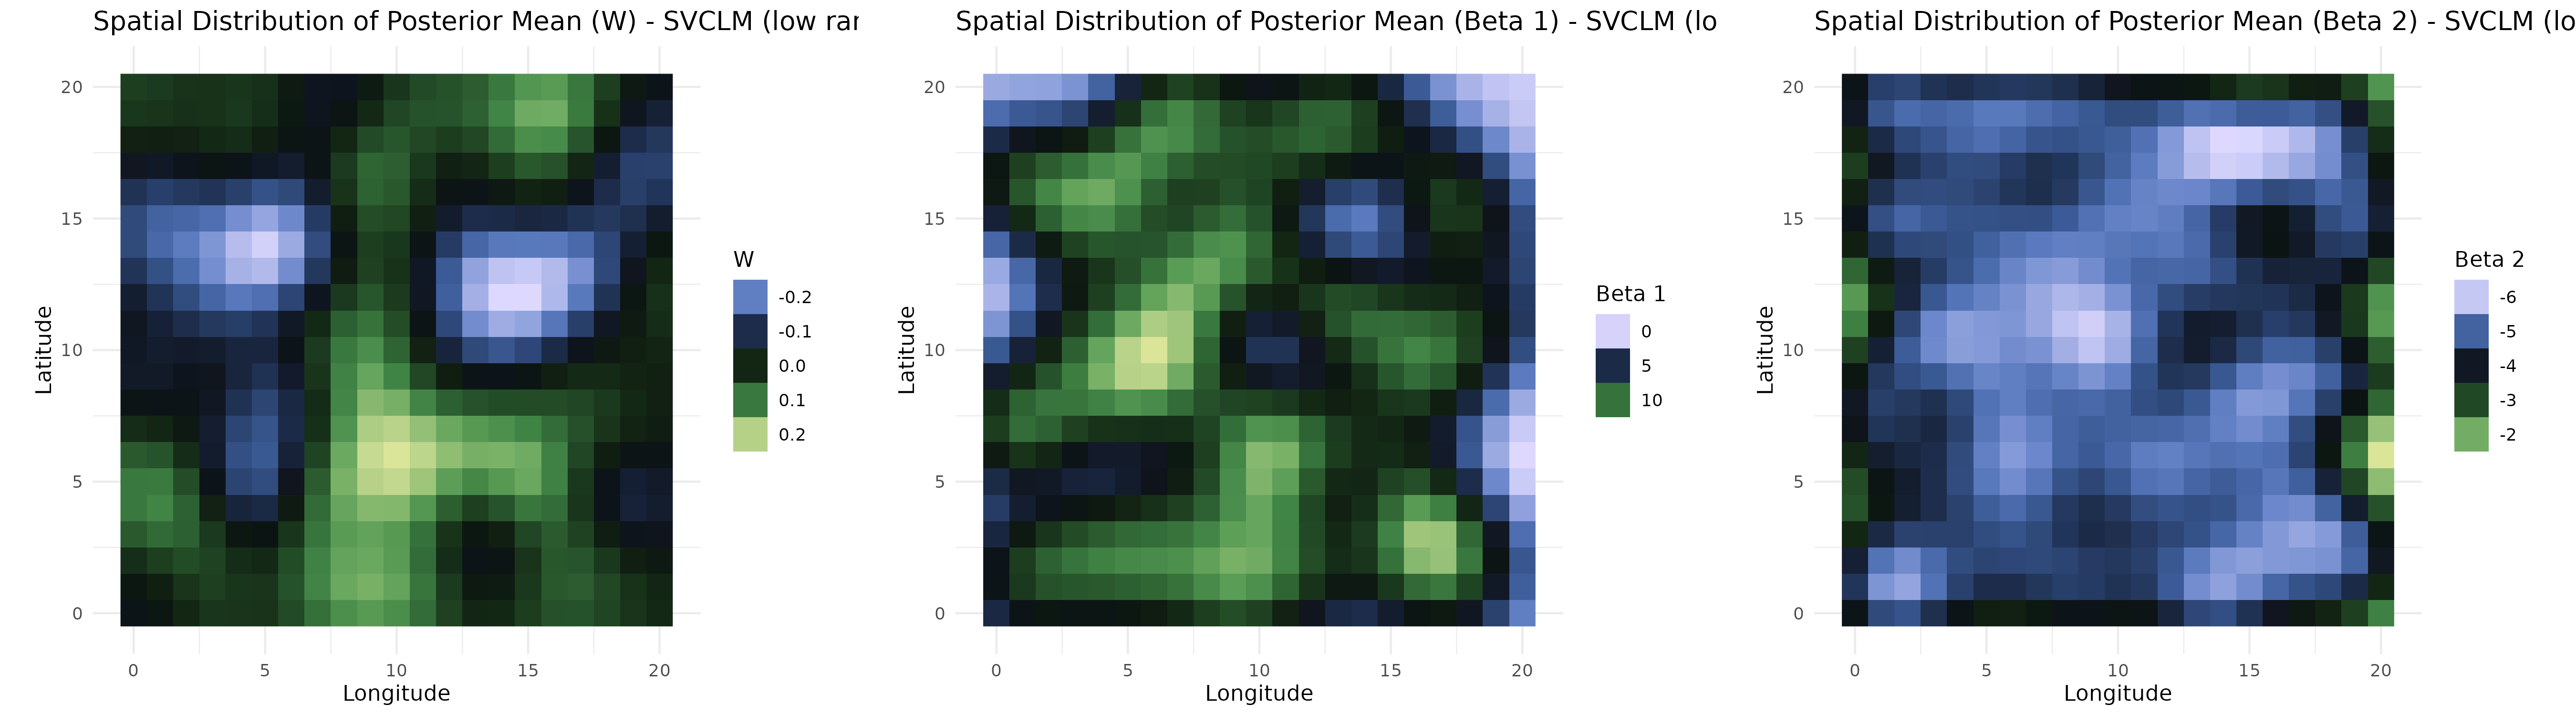
\includegraphics[width=\textwidth]{../../figures/SVCLM_sim.png}
 \caption{Posterior Mappings for Coefficients - SVCLM low rank}
 \label{fig:SVCLMA}
 \end{figure}


\begin{figure}[ht]
 \centering
 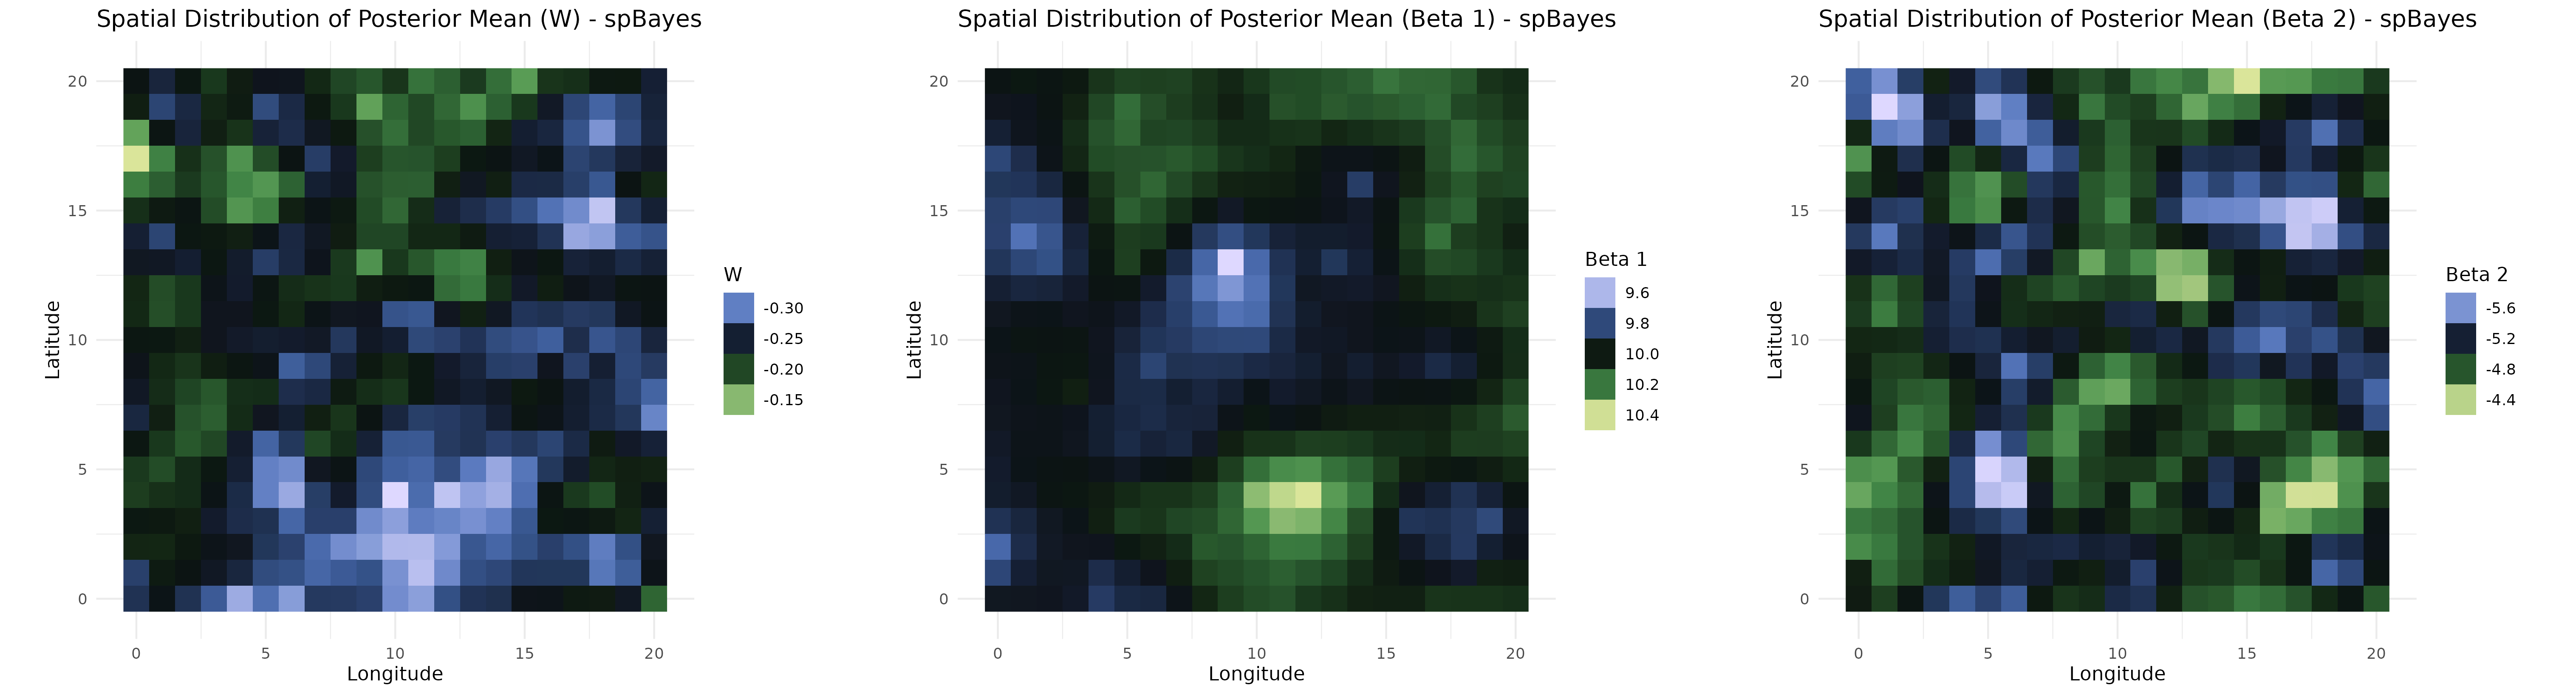
\includegraphics[width=\textwidth]{../../figures/spBayes_sim.png}
 \caption{Posterior Mappings for Coefficients - spBayes}
 \label{fig:spBayesA}
 \end{figure}

\section{Data Analysis}
\label{sec:data analysis}
The real world data used in this section is a gridded satellite data with latitude, longitude, temperature, Normalized Difference Vegetation Index (NDVI); which measures vegetation health/greenness, and emissivity which represents a surface's efficiency in emitting thermal radiation. We used temperature as a univariate outcome and used emissivity and NDVI as covariates.
Figure \ref{fig:spatialpatterns} below reveals the spatial  distributions of the variables in the dataset.

 \begin{figure}[ht]
 \centering
 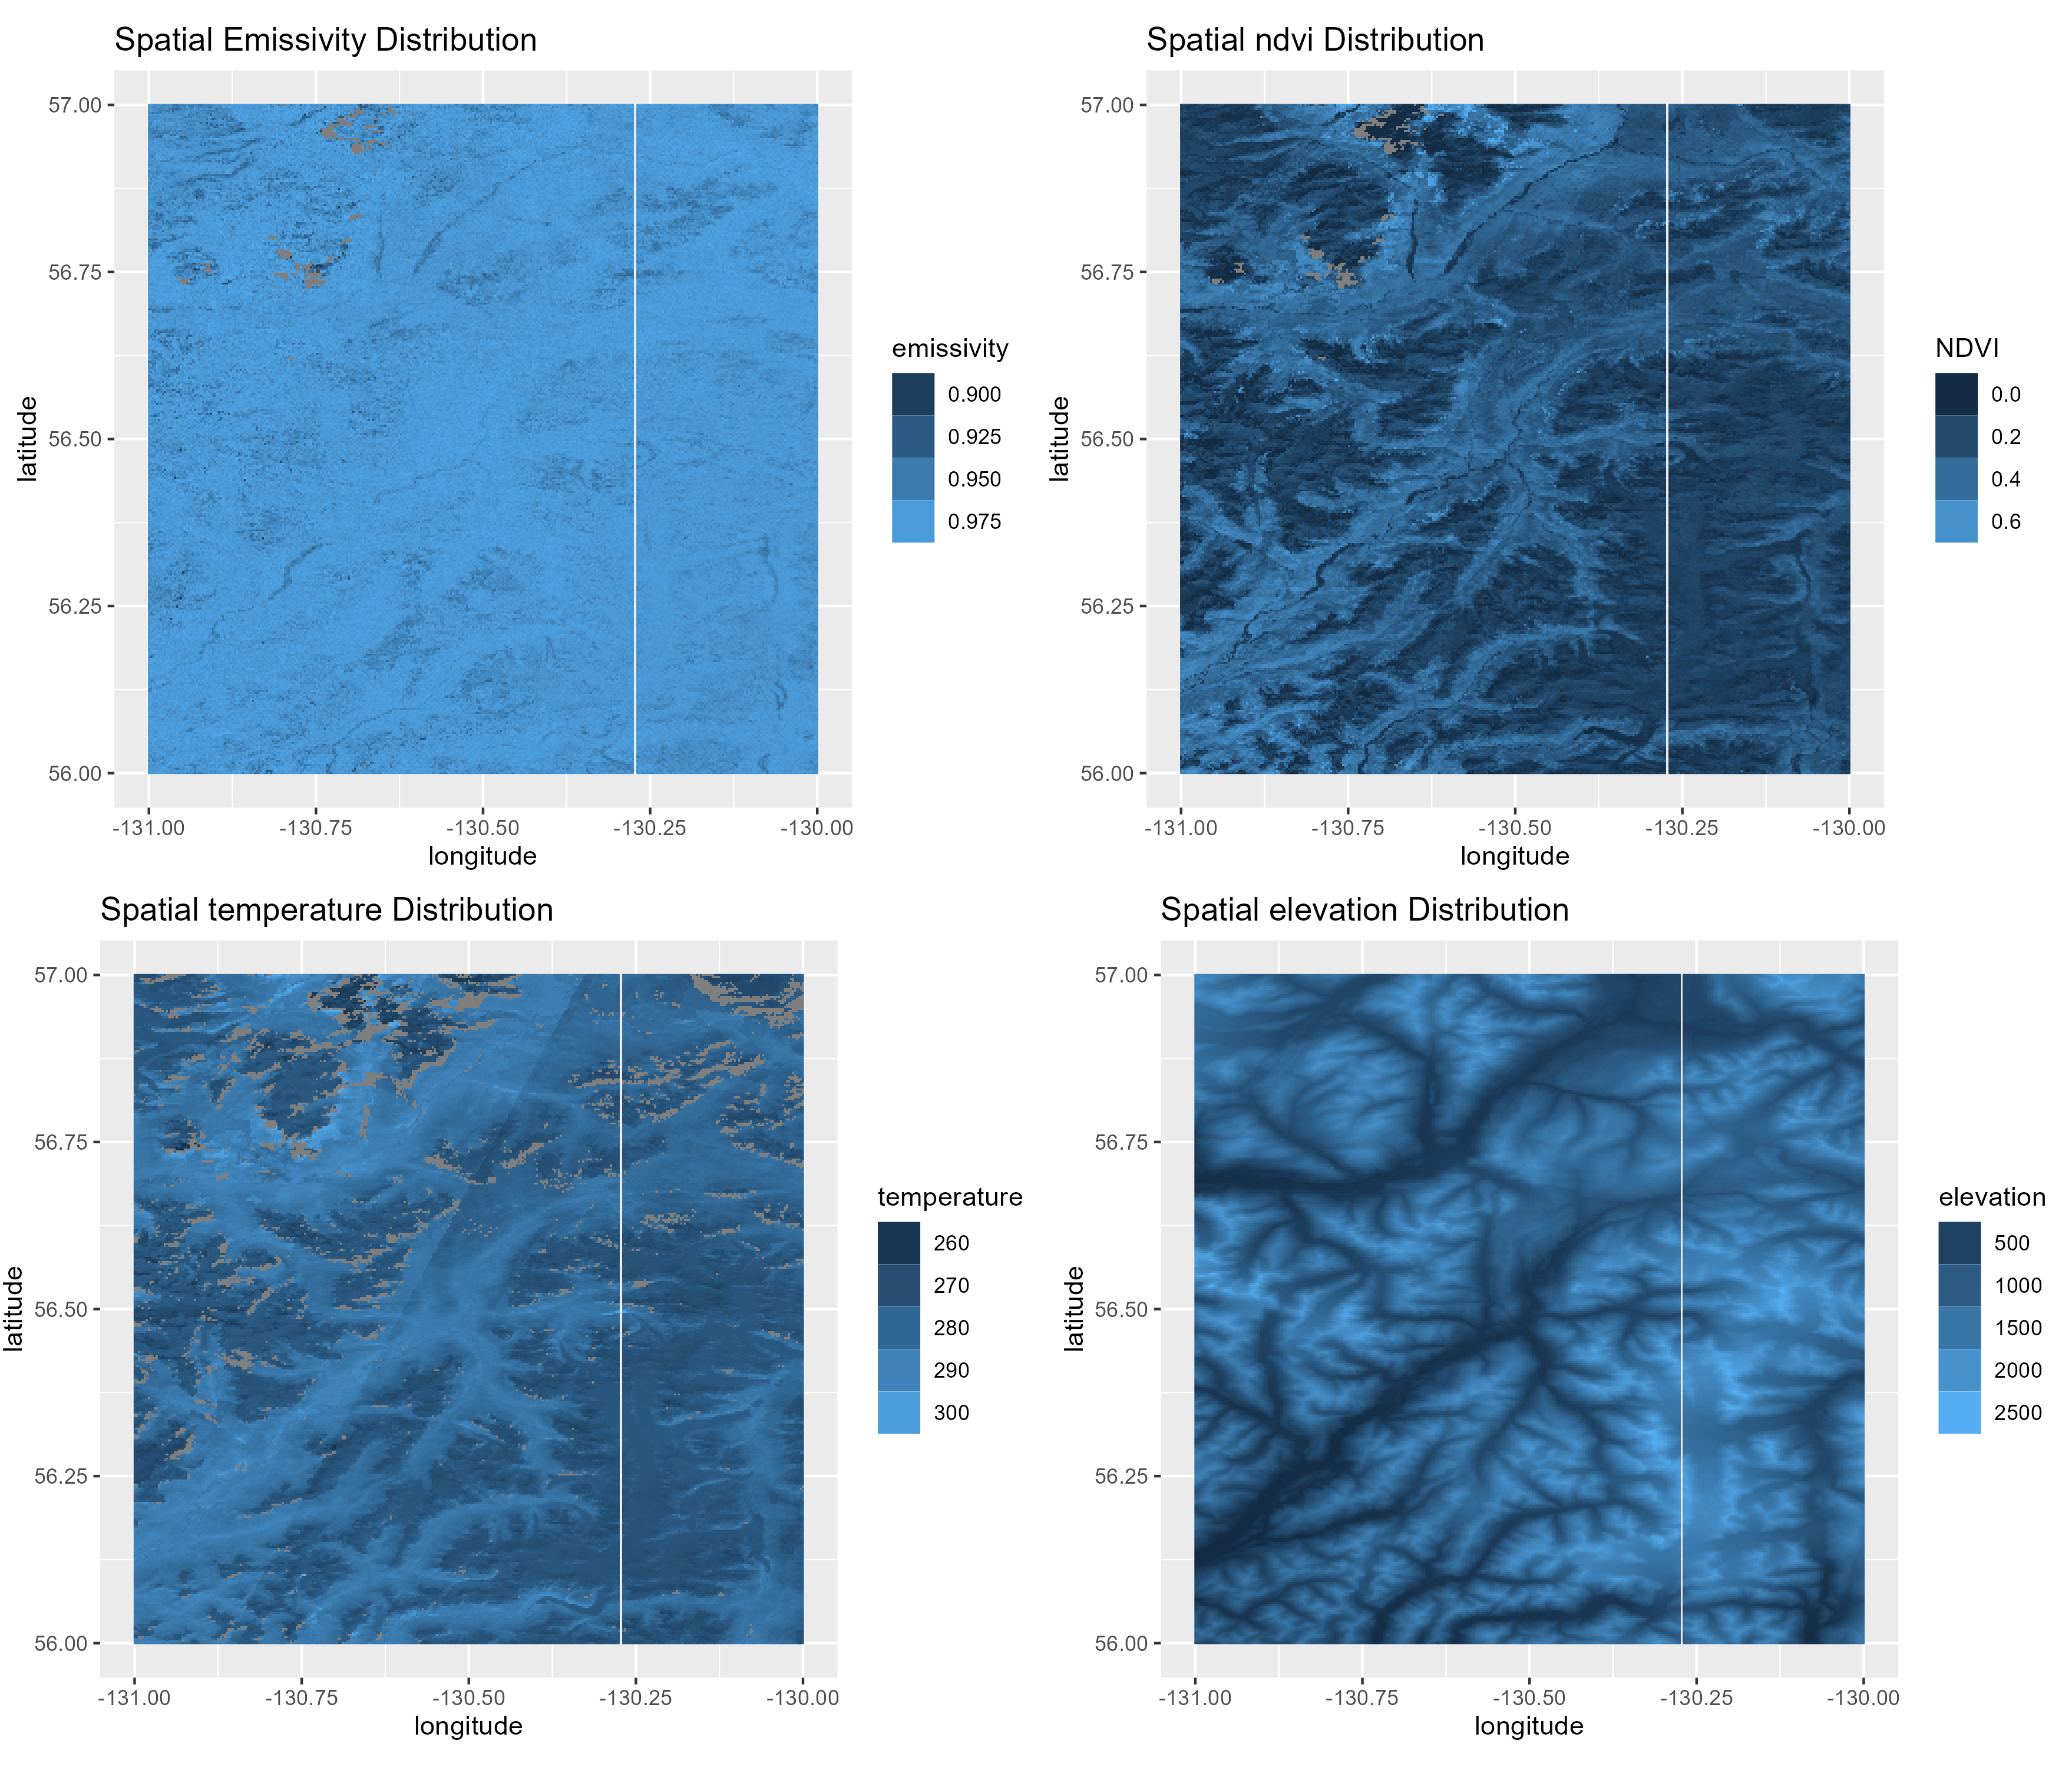
\includegraphics[width=\textwidth]{../../figures/spatial_horizontal_stack.png}
 \caption{
   Spatial distributions of emissivity, NDVI, and  land surface temperature in the study area. 
 }
 \label{fig:spatialpatterns}
 \end{figure}
 
 Emissivity ranges from 0.88 to 0.96. Light blue zones $(\epsilon > 0.94)$ displays dense vegetation/water bodies (high thermal emission efficiency)
 while dark blue clusters $(\epsilon \approx 0.88-0.90)$ represents urbanized areas. Notice that notice that areas with high NDVI also tend to have higher emissivity which makes sense because vegetation emits efficiently.
 Cooler regions often align with greener (higher NDVI) areas — vegetation can reduce surface temperature through evapotranspiration. \newline
 We computed the empirical semivariograms for the variables in the dataset. 
 \begin{figure}[ht]
 \centering
 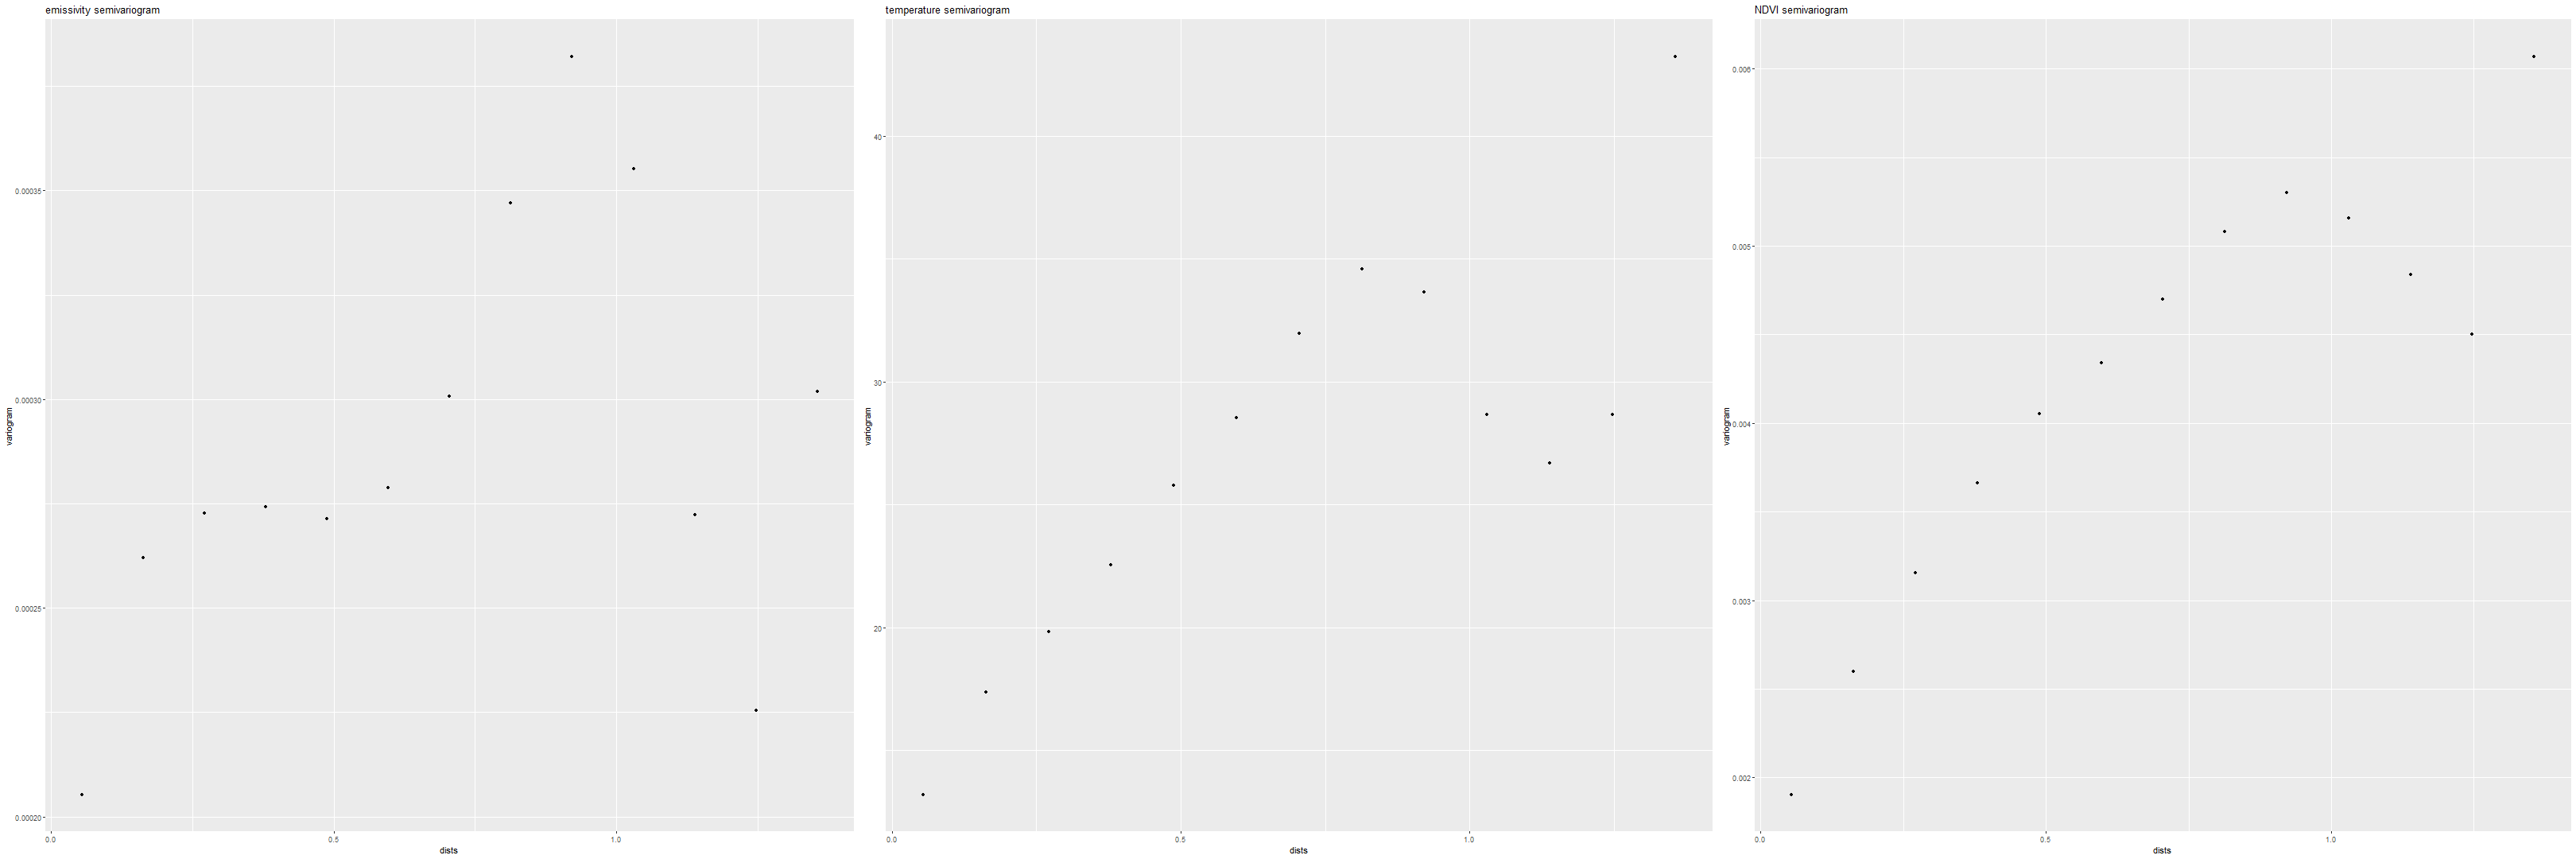
\includegraphics[width=\textwidth]{../../figures/semivariograms.png}
 \caption{Empirical semivariograms for emissivity, temperature and NDVI}
 \label{fig:semivariograms}
 \end{figure}
The variables showed moderate spatial autocorrelation with low to moderate variance.
\subsection{Model}

\subsection{Model fitting}
\textbf{Model Specification}\newline
We modeled land surface temperature (LST) using a spatially varying coefficient (SVC) framework:

\begin{align}
\text{Temp}(s) &= \beta_0(s) + \beta_{\text{NDVI}}(s)\cdot\text{NDVI} + \beta_{\text{Emis}}(s)\cdot\text{Emissivity} + \epsilon(s) \
\epsilon(s) &\sim \text{N}(0, \tau^2) \newline
\beta_r(s) &\sim \text{GP}(0, \sigma_r^2 \exp(-\phi_r^{-1}|s-s'|^2)) \quad \text{for } r \in {0, \text{NDVI}, \text{Emis}}
\end{align}

\textbf{Prior specifications:} We specified weakly informative priors. Spatial variance; $\sigma_r^2 \sim \text{Inv-Gamma}(0.001, 0.001)$.   Spatial range; $\phi_r \sim \text{Uniform}(0.001, 500)$ and  the nugget effect; $\tau^2 \sim \text{Inv-Gamma}(0.001, 0.001)$ \newline
The computational implementation featured Knot-based Approximation. We selected 1 knot per 10 grid cells ($k=10$) using the  $\texttt{simpleknots()}$ function. Removed knots with missing data.
\subsection{Results}
\textbf{Convergence Diagnostics}\newline
We made trace plots after burn-in to check for convergence. 

\begin{figure}[ht]
 \centering
 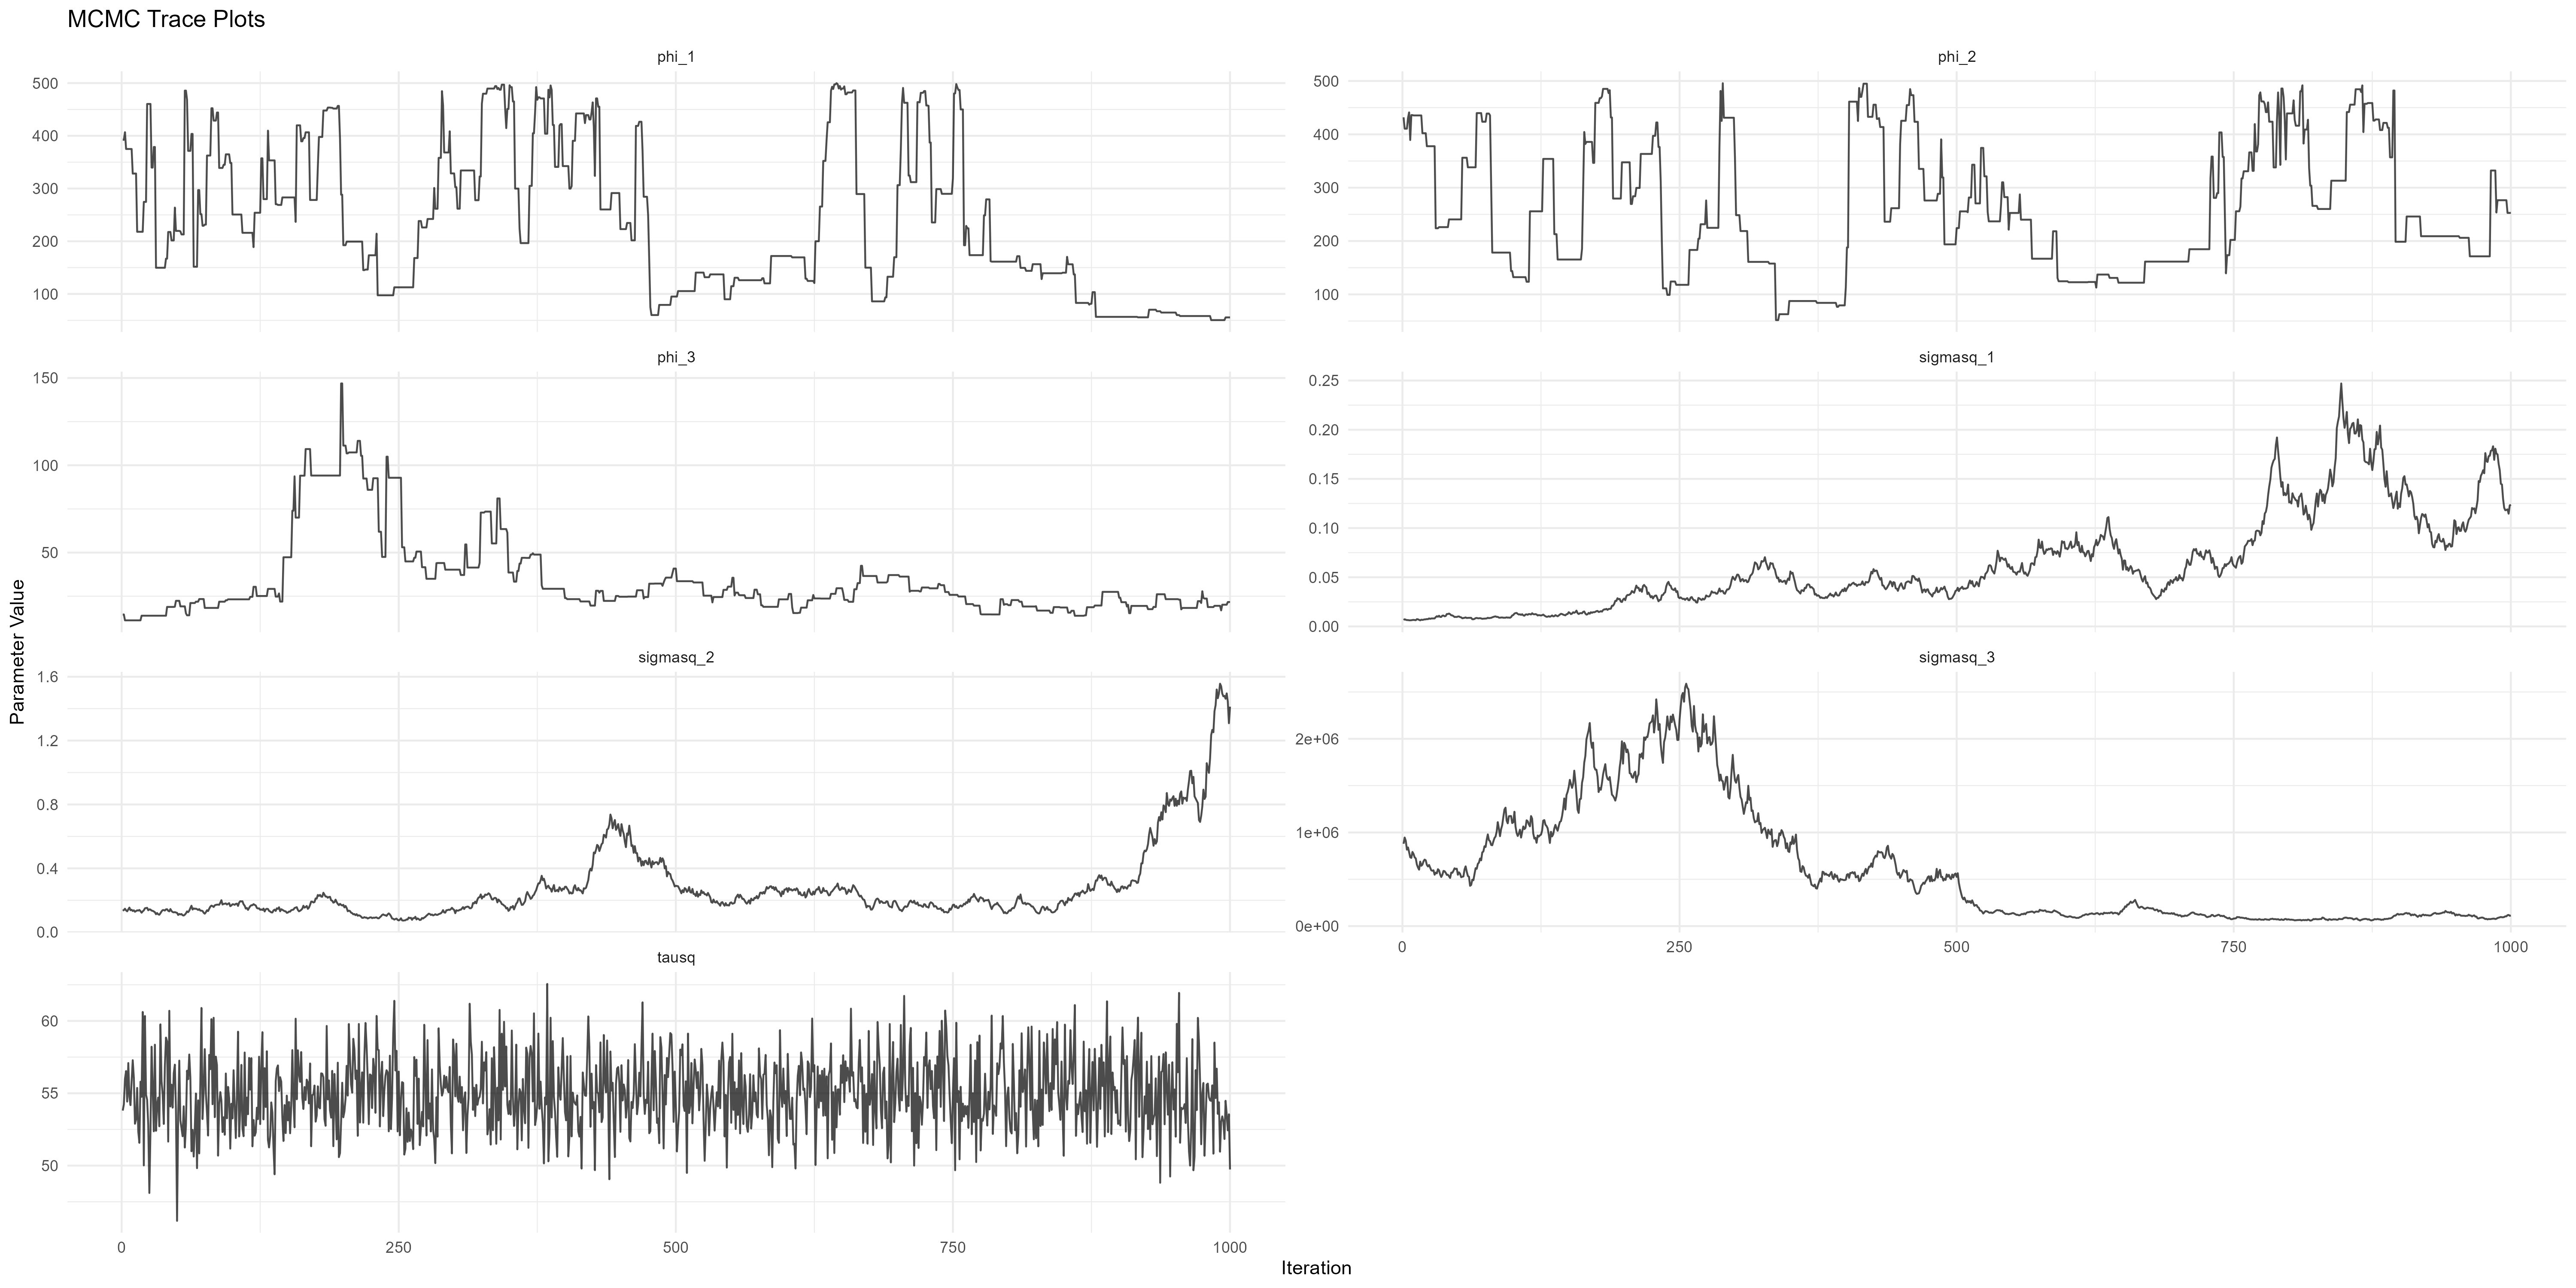
\includegraphics[width=\textwidth]{../../figures/traceplots.png}
 \caption{Trace plots for the parameters in the model}
 \label{fig:traceplots}
 \end{figure}
Some variables display stable and well-mixed behavior, suggesting convergence, while others show trends or irregular jumps which was expected in our setting.

\textbf{Interpretation of Coefficient Surfaces} \newline
Below is a plot of the posterior means of the coefficients over space.

\begin{figure}[ht]
 \centering
 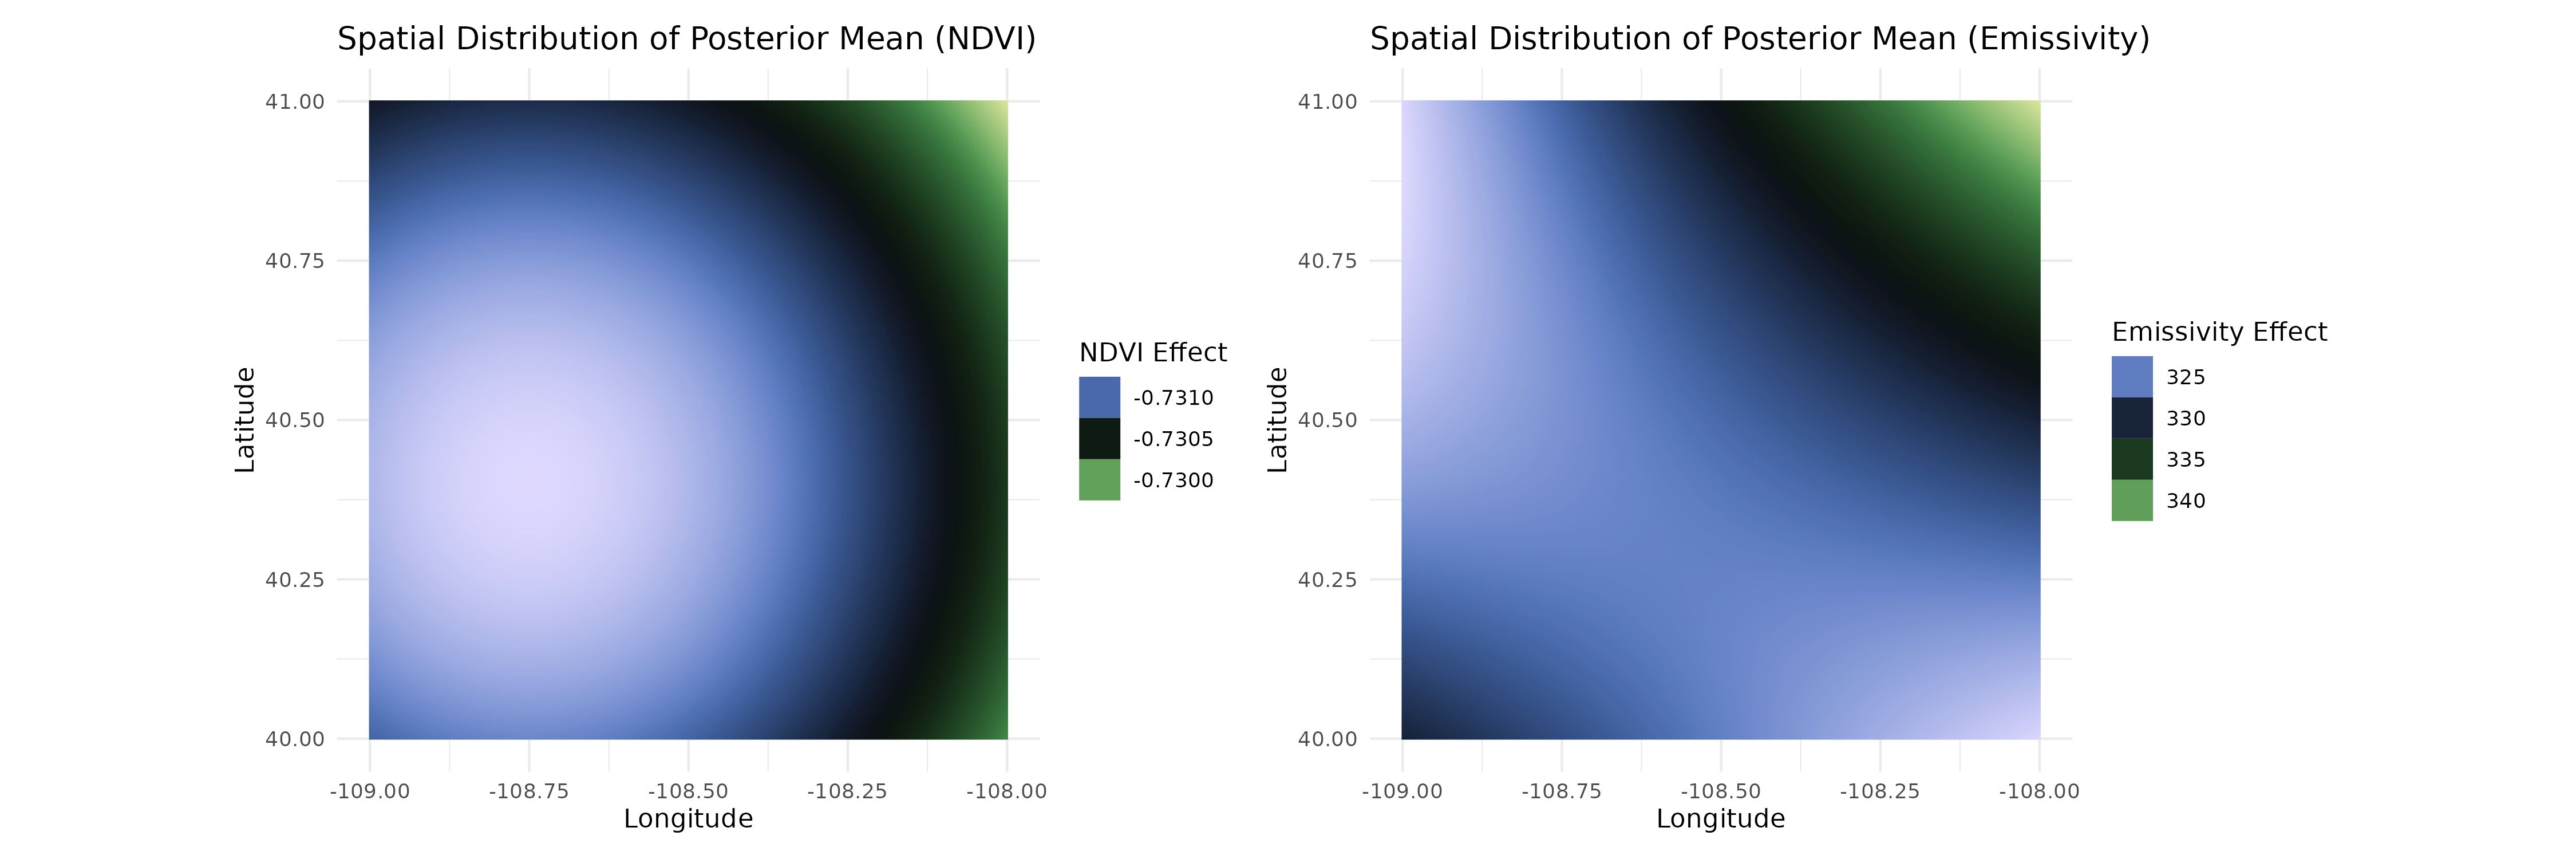
\includegraphics[width=\textwidth]{../../figures/model_means.png}
 \caption{Spatially varying coefficient surfaces for (A) NDVI and (B) Emissivity effects on land surface temperature}
 \label{fig:posterior means}
 \end{figure}
 The posterior mean NDVI coefficients show Strong negative effects (cooling) across the entire study region, with values ranging from -0.7310 to -0.7300. 
 Each unit increase in NDVI corresponds to about $0.73^\circ C$ decrease in land surface temperature across space.
 The emissivity coefficients reveal strong positive associations (mean $\beta_{emis} \approx 330$) which implies that across space, a unit increase in emissivity increase temperature.\newline
 
 
 \textbf{Predctions} \newline
 We generated predicted temperature values across the entire spatial domain using the posterior mean estimates of the spatially varying coefficients. 
 These predictions were computed for all locations with complete predictor data, regardless of whether the actual temperature was observed. 
 The predicted values were obtained by multiplying the mean coefficient estimates with the corresponding covariate values at each location. 
 We then visualized both the observed and predicted temperature surfaces side by side to assess model performance and spatial prediction accuracy. 
 
 
 \begin{figure}[ht]
 \centering
 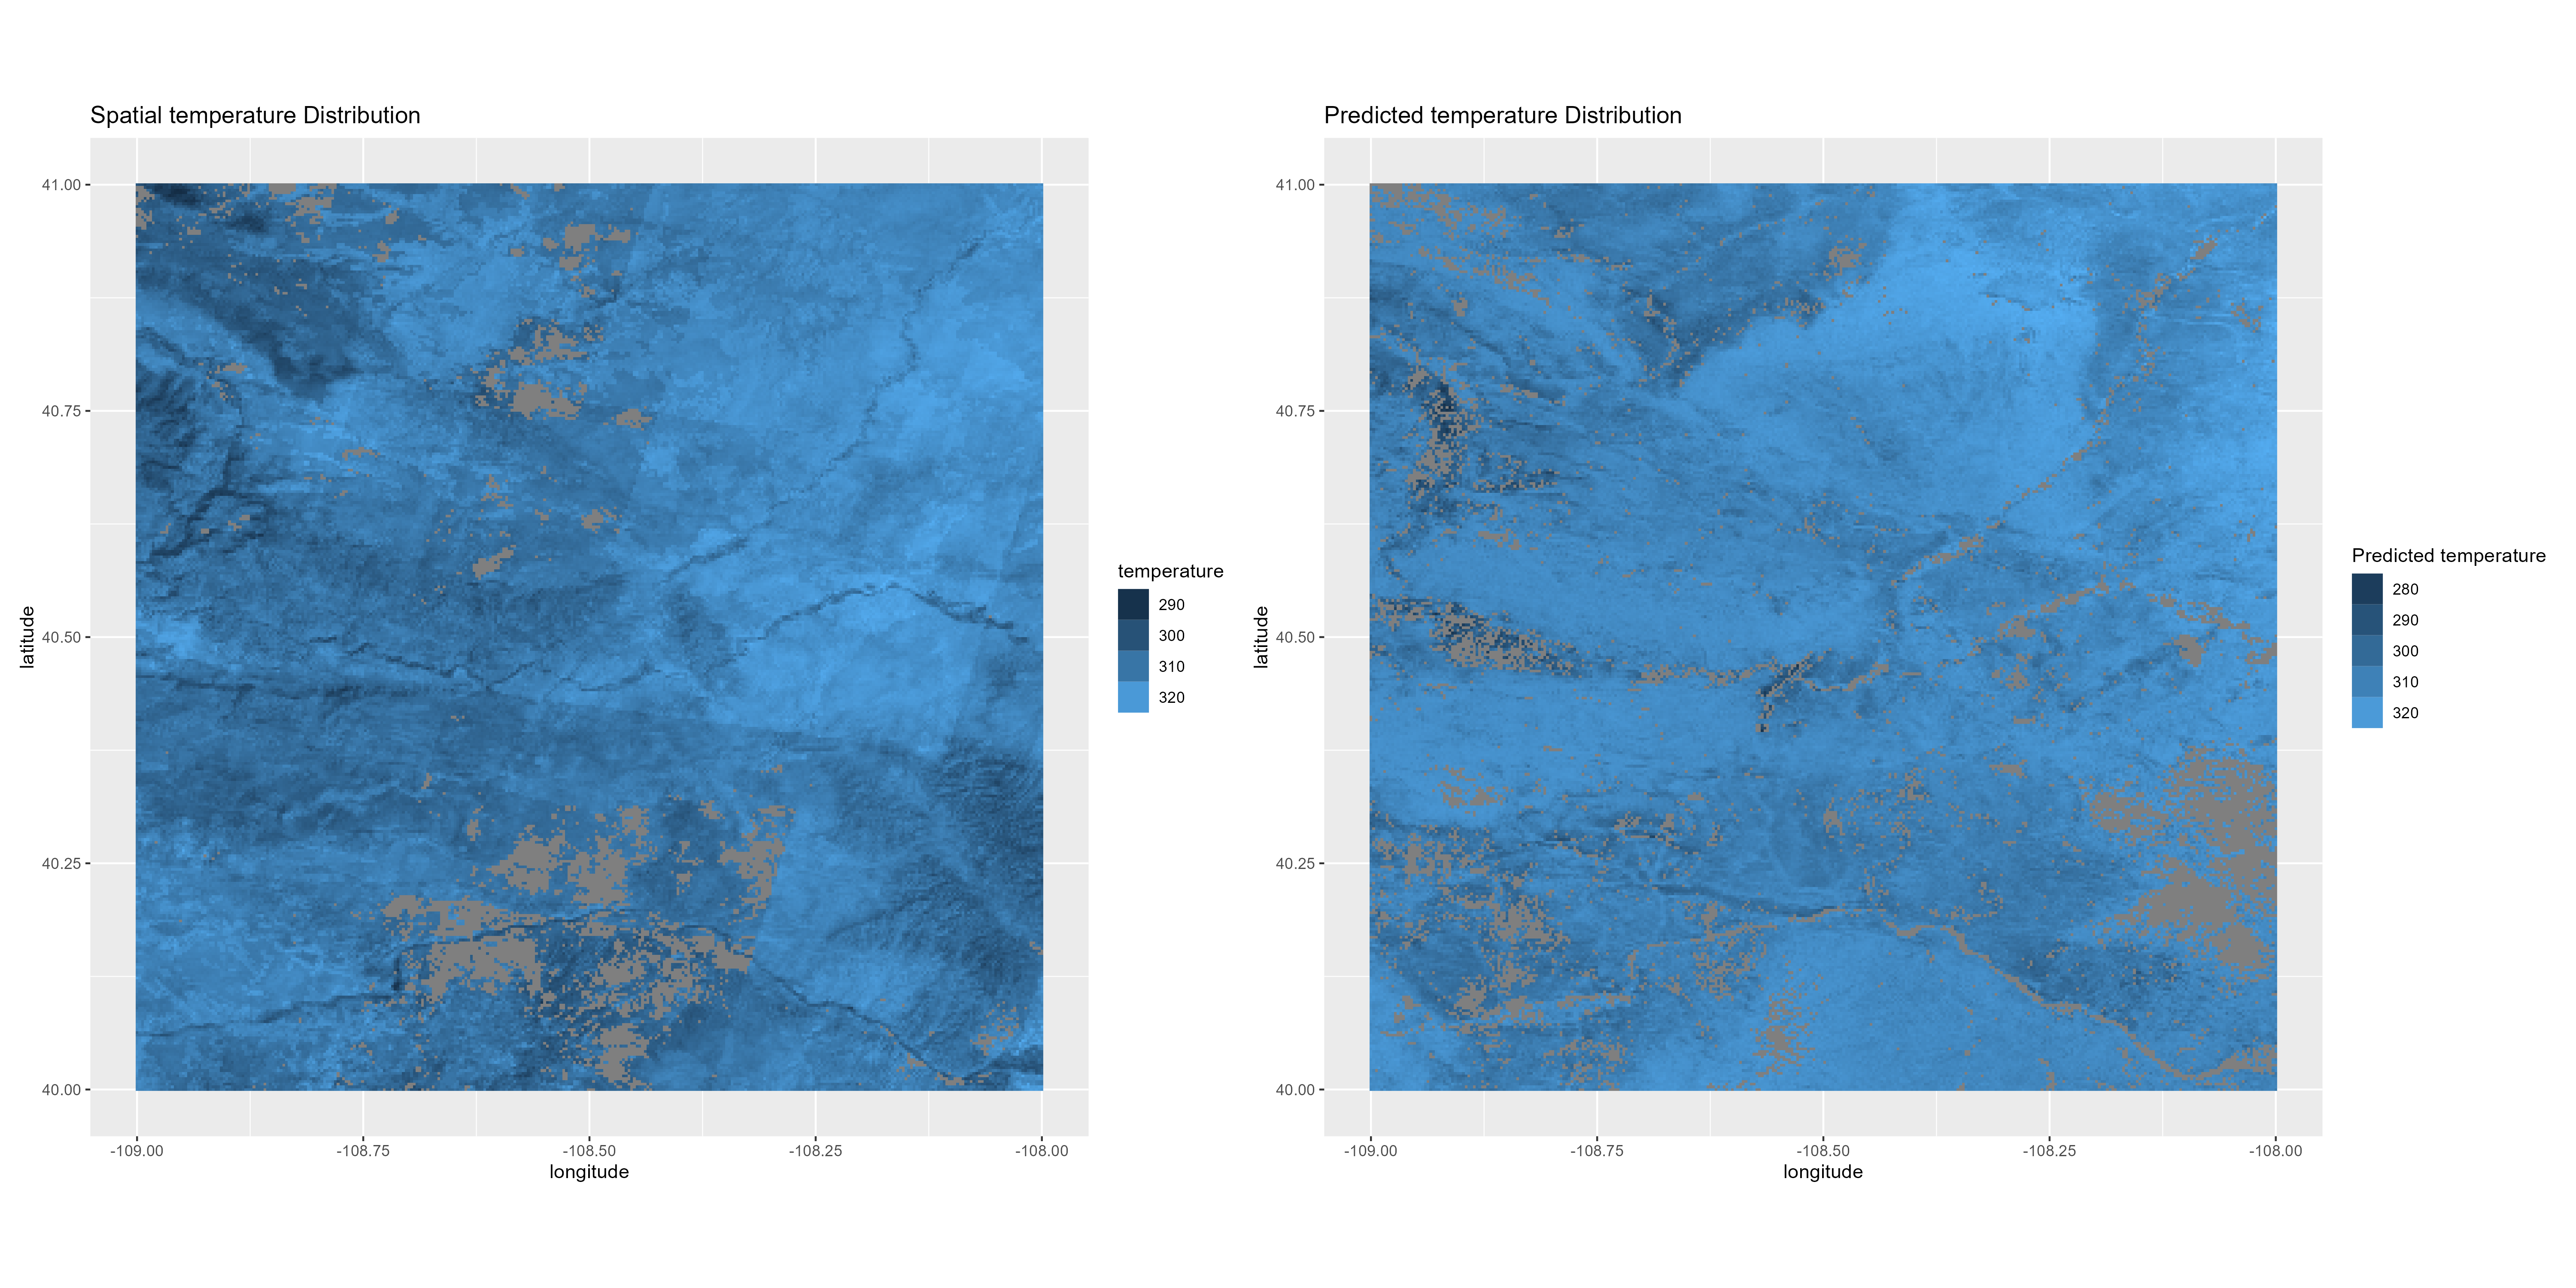
\includegraphics[width=\textwidth]{../../figures/predictions.png}
 \caption{Side by side plot of tempearture and their predicted values across space}
 \label{fig:predicted temperature}
 \end{figure}
 
 The comparison reveals the model’s ability to capture spatial patterns in temperature, even in regions where observations were missing but predictor data were available.
 
 
\section{Conclusion}
Conclusion 

\newpage

\bibliographystyle{agsm}

\bibliography{bibliography}
\end{document}
